\documentclass[12pt,a4paper]{article}

% ─── Page Layout ───────────────────────────────────────────────────────────────
\usepackage[a4paper, margin=0.8in, headheight=14pt]{geometry}

% ─── Fonts (XeLaTeX) ───────────────────────────────────────────────────────────
\usepackage{fontspec}
\usepackage{unicode-math}
\setmainfont{TeX Gyre Pagella}
\setmonofont[Scale=0.88]{TeX Gyre Cursor}
\setmathfont{Latin Modern Math}

% ─── Packages ──────────────────────────────────────────────────────────────────
\usepackage{xcolor}
\usepackage{colortbl}
\usepackage{titlesec}
\usepackage{enumitem}
\usepackage{tabularx}
\usepackage{booktabs}
\usepackage{array}
\usepackage{amsmath}
\usepackage{tikz}
\usetikzlibrary{shapes.geometric, arrows.meta, positioning, calc, fit, decorations.pathreplacing}
\usepackage{tcolorbox}
\tcbuselibrary{skins, breakable}
\usepackage{hyperref}
\usepackage{fancyhdr}
\usepackage{graphicx}
\usepackage{microtype}
\hyphenpenalty=10000
\exhyphenpenalty=10000
\sloppy
\usepackage{caption}
\usepackage{setspace}
\usepackage{multirow}
\usepackage{tocloft}

% ─── Q&A helper ────────────────────────────────────────────────────────────────
\newcommand{\Q}[1]{\textbf{#1}\par\noindent\ignorespaces}

% ─── Colour Palette ────────────────────────────────────────────────────────────
\definecolor{myred}{RGB}{196,30,58}
\definecolor{mydark}{RGB}{30,30,50}
\definecolor{mygreen}{RGB}{14,120,80}
\definecolor{myteal}{RGB}{0,130,140}
\definecolor{myamber}{RGB}{180,100,0}
\definecolor{mypurple}{RGB}{100,30,160}
\definecolor{mygray}{RGB}{246,247,249}
\definecolor{mgframe}{RGB}{180,185,200}
\definecolor{watermark}{RGB}{145,150,170}
\definecolor{hdrred}{RGB}{250,232,235}
\definecolor{hdrgreen}{RGB}{220,244,233}
\definecolor{hdrteal}{RGB}{220,242,244}
\definecolor{hdramber}{RGB}{253,242,215}
\definecolor{hdrpurple}{RGB}{238,228,255}
\definecolor{hdrgray}{RGB}{238,240,245}
\definecolor{rowalt}{RGB}{250,251,253}

% ─── Section Formatting ────────────────────────────────────────────────────────
\titleformat{\section}
  {\large\bfseries\color{myred}}{\thesection.}{0.5em}{}
  [\vspace{1pt}{\color{myred}\rule{\linewidth}{0.8pt}}]
\titleformat{\subsection}
  {\normalsize\bfseries\color{myteal}}{\thesubsection}{0.5em}{}
\titlespacing*{\section}{0pt}{18pt}{7pt}
\titlespacing*{\subsection}{0pt}{11pt}{4pt}

% ─── Paragraph ─────────────────────────────────────────────────────────────────
\setlength{\parindent}{0pt}
\setlength{\parskip}{4pt}

% ─── TOC Styling ───────────────────────────────────────────────────────────────
\renewcommand{\cfttoctitlefont}{\large\bfseries\color{myred}}
\renewcommand{\cftaftertoctitle}{\par\noindent{\color{myred}\rule{\linewidth}{0.8pt}}}
\setlength{\cftbeforetoctitleskip}{0pt}
\setlength{\cftaftertoctitleskip}{6pt}
\renewcommand{\cftsecfont}{\normalsize\bfseries\color{mydark}}
\renewcommand{\cftsecpagefont}{\normalsize\bfseries\color{mydark}}
\renewcommand{\cftsecleader}{\cftdotfill{\cftdotsep}}
\setlength{\cftbeforesecskip}{7pt}
\renewcommand{\cftsubsecfont}{\small\color{mydark}}
\renewcommand{\cftsubsecpagefont}{\small\color{mydark}}
\setlength{\cftbeforesubsecskip}{3pt}
\setlength{\cftsubsecindent}{1.4em}

% ─── Table helpers ─────────────────────────────────────────────────────────────
\renewcommand{\arraystretch}{1.45}
\setlength{\tabcolsep}{6pt}
\arrayrulecolor{mydark}
\newcolumntype{B}[1]{>{\small\bfseries\raggedright\arraybackslash}m{#1}}
\newcolumntype{Y}{>{\small\raggedright\arraybackslash}X}
\renewcommand{\tabularxcolumn}[1]{m{#1}}

% ─── Header / Footer ───────────────────────────────────────────────────────────
\pagestyle{fancy}
\fancyhf{}
\fancyhead[L]{\small\color{myred}\textbf{OE-EC604A}\;\color{mydark}--- Electronic Measurement \& Instruments}
\fancyhead[R]{\small\color{myteal}\textbf{Module 5 Notes}}
\fancyfoot[C]{\small\color{mydark}\thepage}
\fancyfoot[R]{\small\color{watermark}\textit{\copyright\ Biraj}}
\renewcommand{\headrulewidth}{0.5pt}
\renewcommand{\footrulewidth}{0.3pt}

% ─── Hyperref ──────────────────────────────────────────────────────────────────
\hypersetup{
  colorlinks=true, linkcolor=myteal, urlcolor=myteal,
  pdfauthor={Biraj Sarkar},
  pdftitle={OE-EC604A --- Module 5 Notes}
}

% ─── tcolorbox styles ──────────────────────────────────────────────────────────
\tcbset{
  tikzbox/.style={
    colback=mygray, colframe=mgframe, boxrule=0.6pt, arc=4pt,
    left=8pt, right=8pt, top=6pt, bottom=6pt,
    colbacktitle=mgframe, coltitle=mydark,
    fonttitle=\small\bfseries
  },
  defbox/.style={
    colback=hdrgreen, colframe=mygreen, boxrule=0.8pt, arc=4pt,
    left=9pt, right=9pt, top=6pt, bottom=6pt,
    colbacktitle=mygreen, coltitle=white,
    fonttitle=\small\bfseries
  },
  formulabox/.style={
    colback=hdrteal, colframe=myteal, boxrule=0.8pt, arc=4pt,
    left=9pt, right=9pt, top=7pt, bottom=7pt,
    colbacktitle=myteal, coltitle=white,
    fonttitle=\small\bfseries
  },
  examplebox/.style={
    colback=hdramber, colframe=myamber, boxrule=0.8pt, arc=4pt,
    left=9pt, right=9pt, top=6pt, bottom=6pt,
    colbacktitle=myamber, coltitle=white,
    fonttitle=\small\bfseries
  },
  masonbox/.style={
    colback=hdrpurple, colframe=mypurple, boxrule=0.8pt, arc=4pt,
    left=9pt, right=9pt, top=6pt, bottom=6pt,
    colbacktitle=mypurple, coltitle=white,
    fonttitle=\small\bfseries
  },
  exambox/.style={
    colback=hdrpurple, colframe=mypurple, boxrule=1pt, arc=5pt,
    left=10pt, right=10pt, top=8pt, bottom=8pt,
    colbacktitle=mypurple, coltitle=white,
    fonttitle=\bfseries,
    breakable, title after break={\textbf{Frequently Asked / Viva Questions (contd.)}}}
}
% Make all boxes breakable across pages
\tcbset{breakable}

% ─── TikZ styles ───────────────────────────────────────────────────────────────
\tikzset{
  block/.style={rectangle, draw=myteal, fill=hdrteal,
    text width=2.4cm, align=center, minimum height=0.95cm,
    font=\small, rounded corners=3pt, line width=0.7pt},
  redblock/.style={rectangle, draw=myred, fill=hdrred,
    text width=2.4cm, align=center, minimum height=0.95cm,
    font=\small, rounded corners=3pt, line width=0.7pt},
  greenblock/.style={rectangle, draw=mygreen, fill=hdrgreen,
    text width=2.4cm, align=center, minimum height=0.95cm,
    font=\small, rounded corners=3pt, line width=0.7pt},
  amberblock/.style={rectangle, draw=myamber, fill=hdramber,
    text width=2.4cm, align=center, minimum height=0.95cm,
    font=\small, rounded corners=3pt, line width=0.7pt},
  purpblock/.style={rectangle, draw=mypurple, fill=hdrpurple,
    text width=2.4cm, align=center, minimum height=0.95cm,
    font=\small, rounded corners=3pt, line width=0.7pt},
  sumjunc/.style={circle, draw=myamber, fill=hdramber,
    minimum size=0.62cm, font=\small, line width=0.8pt},
  arrow/.style={-Stealth, thick, color=mydark},
  redarrow/.style={-Stealth, thick, color=myred},
  line/.style={thick, color=mydark}
}

% ═══════════════════════════════════════════════════════════════════════════════
\begin{document}
% ═══════════════════════════════════════════════════════════════════════════════

\begin{center}
  {\LARGE\bfseries\color{myred} OE-EC604A --- Electronic Measurement \& Measuring Instruments}\\[5pt]
  {\normalsize\color{mydark} Semester VI \quad$\bullet$\quad 3L:0T:0P \quad$\bullet$\quad 3 Credits}\\[3pt]
  {\normalsize\color{myteal}\textbf{Module 5 Exam Notes: Bridges, Parameter Measurement \& DAS}}\\[3pt]
  {\small\color{mydark} CGEC \;$|$\; B.Tech ECE (2023--27) \;$|$\; \textit{Biraj Sarkar}}
\end{center}
\vspace{2pt}
\noindent{\color{myred}\rule{\linewidth}{1.5pt}}
\vspace{2pt}

\hypersetup{linkcolor=mydark}
\tableofcontents
\hypersetup{linkcolor=myteal}
\newpage

% ===============================================================================
\section{DC and AC Bridges}
% ===============================================================================

Bridges are comparison circuits used to measure resistance, inductance, capacitance, and impedance with high precision.

\subsection{Wheatstone Bridge}
The \textbf{Wheatstone Bridge} is a fundamental DC bridge used for measuring medium resistances ($1\,\Omega$ to $100\,\text{k}\Omega$).

\begin{tcolorbox}[defbox, title={\textbf{Wheatstone Bridge Principle}}]
It consists of four resistive arms forming a closed loop, with a DC source connected across one pair of opposite junctions and a null detector (galvanometer) across the other. When the potential difference across the galvanometer is zero, the bridge is balanced.
\end{tcolorbox}

\subsubsection{Derivation of Balance Equation}
Let the four resistive arms be $P$, $Q$, $R$, and $S$:
\begin{itemize}[leftmargin=*, itemsep=3pt]
  \item $P$ and $Q$ are fixed, known ratio arms.
  \item $R$ is the variable standard resistance.
  \item $S$ is the unknown resistance ($R_x$).
\end{itemize}
At balance, the current through the galvanometer is $I_g = 0$. This implies:
\begin{equation}
  V_B = V_D \implies I_1 P = I_2 R
\end{equation}
Since no current passes through the galvanometer, the current in arm $BC$ is $I_1$ and in arm $DC$ is $I_2$:
\begin{equation}
  I_1 = \frac{E}{P + Q} \qquad \text{and} \qquad I_2 = \frac{E}{R + S}
\end{equation}
Substituting these currents into the potential equation:
\begin{equation}
  \left(\frac{E}{P + Q}\right) P = \left(\frac{E}{R + S}\right) R \implies \frac{P}{P + Q} = \frac{R}{R + S}
\end{equation}
Cross-multiplying yields:
\begin{equation}
  P(R + S) = R(P + Q) \implies P R + P S = P R + Q R \implies P S = Q R \implies S = \frac{Q}{P} R
\end{equation}
Thus, the unknown resistance is:
\begin{equation}
  R_x = \frac{Q}{P} R
\end{equation}

\subsubsection{Limitations of Wheatstone Bridge}
It cannot measure low resistances ($< 1\,\Omega$) accurately because the contact resistances of terminals and the lead wire resistances are of similar magnitude, introducing significant errors.

\subsection{Kelvin Double Bridge}
The \textbf{Kelvin Double Bridge} is a modification of the Wheatstone bridge designed specifically to eliminate lead and contact resistances when measuring low resistances ($1\,\mu\Omega$ to $1\,\Omega$).

\begin{tcolorbox}[defbox, title={\textbf{Kelvin Double Bridge Concept}}]
It introduces a second set of ratio arms ($p$ and $q$) which are connected to a galvanometer to bypass the potential drop across the low-resistance connecting link ($r$) between the unknown low resistance ($R$) and standard low resistance ($S$).
\end{tcolorbox}

\subsubsection{Derivation of Balance Equation}
Let the main ratio arms be $P$ and $Q$, and the inner ratio arms be $p$ and $q$. The resistance of the connecting lead is $r$.
The galvanometer is connected between the junction of $P$ and $Q$ and the junction of $p$ and $q$. At balance, the potential difference across the galvanometer is zero.
The current $I$ divides at the connecting link:
\begin{itemize}[leftmargin=*, itemsep=3pt]
  \item Main branch current is $I$.
  \item The path through the inner ratio arms ($p+q$) is in parallel with the link resistance $r$.
\end{itemize}
The current through the link branch $p+q$ is:
\begin{equation}
  I_{pq} = I \cdot \frac{r}{p + q + r}
\end{equation}
The voltage drop across the branch $p$ is:
\begin{equation}
  V_p = I_{pq} \cdot p = I \left( \frac{p r}{p + q + r} \right)
\end{equation}
For balance, the ratio of potential drops across the primary arms must be equal:
\begin{equation}
  \frac{P}{Q} = \frac{R + V_p}{S + V_q} = \frac{R + I \left(\frac{p r}{p + q + r}\right)}{S + I \left(\frac{q r}{p + q + r}\right)}
\end{equation}
Cross-multiplying and solving for $R$:
\begin{equation}
  P \left[ S + \frac{q r}{p + q + r} \right] = Q \left[ R + \frac{p r}{p + q + r} \right]
\end{equation}
\begin{equation}
  P S + \frac{P q r}{p + q + r} = Q R + \frac{Q p r}{p + q + r}
\end{equation}
\begin{equation}
  Q R = P S + \frac{P q r - Q p r}{p + q + r}
\end{equation}
Dividing by $Q$:
\begin{equation}
  R = \frac{P}{Q} S + \frac{q r}{p + q + r} \left( \frac{P}{Q} - \frac{p}{q} \right)
\end{equation}
If we design the bridge such that the ratio of the inner arms equals the ratio of the outer arms:
\begin{equation}
  \frac{P}{Q} = \frac{p}{q}
\end{equation}
Then the term $\left(\frac{P}{Q} - \frac{p}{q}\right)$ becomes zero. The balance equation simplifies to:
\begin{equation}
  R = \frac{P}{Q} S
\end{equation}
Thus, the effect of the connecting lead resistance $r$ is completely eliminated.

\subsection{Maxwell Inductance-Capacitance Bridge}
The \textbf{Maxwell Bridge} is an AC bridge used to measure an unknown inductance by comparing it with a standard variable capacitor. It is suited for measuring medium-Q coils ($1 < Q < 10$).

\begin{tcolorbox}[tikzbox, title={Maxwell Inductance-Capacitance Bridge Circuit}]
\centering
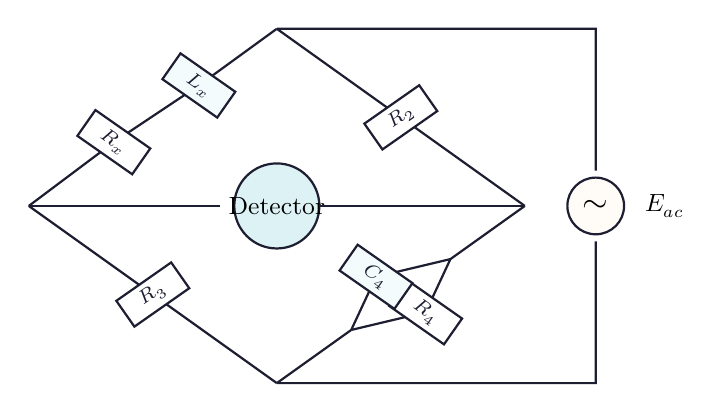
\begin{tikzpicture}[scale=0.9, thick, font=\small, >=Stealth]
  % Define main coordinates
  \coordinate (A) at (0, 2.5);
  \coordinate (B) at (-3.5, 0);
  \coordinate (C) at (0, -2.5);
  \coordinate (D) at (3.5, 0);

  % Draw Detector
  \draw[line] (B) -- (-0.8, 0);
  \draw[draw=mydark, fill=hdrteal] (0, 0) circle (0.6) node {Detector};
  \draw[line] (0.6, 0) -- (D);

  % Helper component node style
  \tikzset{
    comp/.style={rectangle, draw=mydark, fill=white, minimum width=0.85cm, minimum height=0.4cm, inner sep=2pt, font=\scriptsize}
  }

  % Arm AB (Top-Left): Rx and Lx in series
  \draw[line] (B) -- (-2.3, 0.9) node[comp, rotate=-35] (Rx) {$R_x$} -- (-1.1, 1.7) node[comp, fill=hdrteal!30, rotate=-35] (Lx) {$L_x$} -- (A);
  
  % Arm AD (Top-Right): R2
  \draw[line] (A) -- (1.75, 1.25) node[comp, rotate=35] (R2) {$R_2$} -- (D);

  % Arm BC (Bottom-Left): R3
  \draw[line] (B) -- (-1.75, -1.25) node[comp, rotate=35] (R3) {$R_3$} -- (C);

  % Arm DC (Bottom-Right): R4 in parallel with C4
  \coordinate (DCmid) at (1.75, -1.25);
  \draw[line] (D) -- (2.45, -0.75);
  % R4 branch
  \draw[line] (2.45, -0.75) -- (2.1, -1.5) node[comp, rotate=-35] (R4) {$R_4$} -- (1.05, -1.75);
  % C4 branch
  \draw[line] (2.45, -0.75) -- (1.4, -1.0) node[comp, fill=hdrteal!30, rotate=-35] (C4) {$C_4$} -- (1.05, -1.75);
  \draw[line] (1.05, -1.75) -- (C);

  % AC Source Loop
  \draw[line] (A) -- (4.5, 2.5) -- (4.5, 0.5);
  \draw[draw=mydark, fill=hdramber!20] (4.5, 0) circle (0.4) node {\large $\sim$};
  \draw[line] (4.5, -0.5) -- (4.5, -2.5) -- (C);
  \node[right=0.5cm of {4.5,0}, font=\small] {$E_{ac}$};
\end{tikzpicture}
\end{tcolorbox}

\subsubsection{Derivation of Balance Equation}
Let:
\begin{itemize}[leftmargin=*, itemsep=3pt]
  \item Arm 1 ($AB$): Impedance $Z_1 = R_x + j\omega L_x$ (unknown inductance and resistance).
  \item Arm 2 ($AD$): Impedance $Z_2 = R_2$ (non-inductive resistance).
  \item Arm 3 ($BC$): Impedance $Z_3 = R_3$ (non-inductive resistance).
  \item Arm 4 ($DC$): Impedance $Z_4$ consists of $R_4$ in parallel with $C_4$. Thus, its admittance $Y_4$ is:
    \begin{equation}
      Y_4 = \frac{1}{R_4} + j\omega C_4
    \end{equation}
\end{itemize}
The general AC bridge balance condition is:
\begin{equation}
  Z_1 \cdot Z_4 = Z_2 \cdot Z_3 \implies Z_1 = \frac{Z_2 Z_3}{Z_4} = Z_2 Z_3 Y_4
\end{equation}
Substitute the values of $Z_1$, $Z_2$, $Z_3$, and $Y_4$:
\begin{equation}
  R_x + j\omega L_x = R_2 R_3 \left( \frac{1}{R_4} + j\omega C_4 \right)
\end{equation}
\begin{equation}
  R_x + j\omega L_x = \frac{R_2 R_3}{R_4} + j\omega R_2 R_3 C_4
\end{equation}
Equating the real and imaginary parts on both sides:
\begin{equation}
  \text{Real Part:} \quad R_x = \frac{R_2 R_3}{R_4}
\end{equation}
\begin{equation}
  \text{Imaginary Part:} \quad L_x = R_2 R_3 C_4
\end{equation}
The Quality Factor ($Q$) of the inductor is:
\begin{equation}
  Q = \frac{\omega L_x}{R_x} = \frac{\omega (R_2 R_3 C_4)}{\left(\frac{R_2 R_3}{R_4}\right)} = \omega C_4 R_4
\end{equation}

\subsubsection{Advantages and Disadvantages}
\begin{itemize}[leftmargin=*, itemsep=3pt]
  \item \textbf{Advantages:} Balance equations are independent of frequency; simple relation for computing $L_x$ and $R_x$ separately.
  \item \textbf{Disadvantages:} Requires an expensive variable capacitor; not suitable for high-Q coils ($Q > 10$) because the required resistance $R_4$ becomes extremely high, making it impractical.
\end{itemize}

\newpage
% ===============================================================================
\section{Measurement of Non-Electrical Parameters}
% ===============================================================================

\subsection{Flow Measurement: Electromagnetic Flow Meter}
Electromagnetic flow meters measure the volumetric flow rate of an electrically conducting fluid.

\begin{tcolorbox}[defbox, title={\textbf{Working Principle (Faraday's Law)}}]
When a conductive fluid flows through a pipe of diameter $D$ across a transverse magnetic field of flux density $B$, an electromotive force (EMF) $E$ is induced across the electrodes perpendicular to the field:
\begin{equation}
  E = B \cdot D \cdot v
\end{equation}
where $v$ is the average fluid velocity.
\end{tcolorbox}

\subsubsection{Concept and Working}
\begin{itemize}[leftmargin=*, itemsep=3pt]
  \item A magnetic coil placed around the pipe creates a uniform magnetic field.
  \item As the conductive fluid (measurand) flows, it acts as a moving conductor, generating voltage.
  \item Metallic electrodes flush-mounted on the pipe walls pick up the induced voltage.
  \item The flow rate $Q$ is proportional to velocity: $Q = A \cdot v = \frac{\pi D^2}{4} \cdot \left(\frac{E}{B D}\right) = \frac{\pi D}{4 B} \cdot E \implies Q \propto E$.
\end{itemize}
- \textbf{Advantages:} Non-invasive (zero pressure drop), handles corrosive/slurry liquids, independent of viscosity, density, and temperature.
- \textbf{Disadvantages:} Fluid must be electrical-conducting ($> 5\,\mu\text{S/cm}$); cannot measure oil, gas, or pure water.

\subsection{Level Measurement}
\subsubsection{Capacitive Level Transducer}
Operates on the variation of capacitance between two concentric cylindrical electrodes placed in a vessel.
- \textbf{Non-Conducting Fluid:} Capacitance changes as the liquid level $h$ rises, displacing air:
  \begin{equation}
    C = \frac{2\pi\epsilon_0 [h\epsilon_r + (H - h)]}{\ln(b/a)}
  \end{equation}
  where $a$ and $b$ are the inner and outer electrode radii, $H$ is the total height, and $\epsilon_r$ is the liquid dielectric constant.
- \textbf{Conducting Fluid:} The probe is insulated with a thin dielectric material (e.g., Teflon). The fluid acts as the outer plate of the capacitor. The capacitance varies linearly with depth $h$.

\subsubsection{Ultrasonic Level Transducer}
Non-contact type sensor mounted at the top of the tank.
- \textbf{Working:} Emits ultrasonic pulses downward. The pulses reflect off the liquid surface and return to the transducer.
- \textbf{Formula:} The distance to the liquid surface $d$ is calculated from transit time $t$:
  \begin{equation}
    d = \frac{v \cdot t}{2} \qquad (\text{where } v = \text{velocity of sound in air})
  \end{equation}
  The liquid level is $h = H - d$, where $H$ is the total height of the tank.

\subsection{Pressure Measurement}
\subsubsection{LVDT-Based Pressure Cell}
A mechanical pressure-sensing element (bellows, diaphragm, or Bourdon tube) is used as the primary transducer to convert pressure into physical displacement. The core of an LVDT is connected to this element as the secondary transducer, converting displacement into an electrical output voltage.

\subsubsection{Pirani Vacuum Gauge}
A thermal conductivity gauge used to measure low pressures ($10^{-4}\,\text{torr}$ to $1\,\text{torr}$).
- \textbf{Working:} A heated tungsten filament is placed in a chamber connected to the vacuum system. As pressure decreases, the density of gas molecules decreases. Fewer molecules collide with the filament, reducing heat dissipation (thermal conductivity drops). The filament temperature increases, raising its electrical resistance. This resistance change is measured using a Wheatstone bridge.

\subsubsection{McLeod Vacuum Gauge}
An absolute calibration instrument used to measure very low pressures down to $10^{-6}\,\text{torr}$.
- \textbf{Working:} A gas sample of large initial volume $V$ at unknown low pressure $P$ is compressed into a small capillary tube of area $a$ to a much smaller volume. The compressed pressure is measured using a mercury column height difference $h$.
- \textbf{Formula:} Applying Boyle's Law ($P_1 V_1 = P_2 V_2$):
  \begin{equation}
    P \cdot V = (P + h) \cdot (a \cdot h)
  \end{equation}
  Since $P \ll h$ under compression, the unknown pressure is approximated as:
  \begin{equation}
    P \approx \frac{a \cdot h^2}{V}
  \end{equation}


\subsection{Humidity and Moisture Measurement}
Humidity indicates the water vapor content in the air, while moisture refers to the water content bound inside materials (e.g., soil, grains, wood).

\begin{tcolorbox}[defbox, title={\textbf{Relative Humidity (RH)}}]
Relative Humidity (RH) is the ratio of the actual water vapor pressure ($p_v$) to the saturation water vapor pressure ($p_s$) of air at the same temperature, expressed as a percentage:
\begin{equation}
  \text{RH} = \frac{p_v}{p_s} \times 100\%
\end{equation}
\end{tcolorbox}

\subsubsection{Sling Psychrometer (Wet/Dry Bulb Principle)}
A sling psychrometer is a classical instrument used to measure relative humidity by comparing dry-bulb and wet-bulb temperatures.
\begin{itemize}[leftmargin=*, itemsep=3.5pt]
  \item \textbf{Working Principle:} It consists of two identical thermometers mounted side-by-side:
    \begin{itemize}[leftmargin=*, itemsep=2.5pt, topsep=0pt]
      \item \textbf{Dry-Bul Thermometer ($T_d$):} Exposed directly to ambient air to measure standard dry air temperature.
      \item \textbf{Wet-Bul Thermometer ($T_w$):} Its bulb is covered with a clean cotton wick saturated with distilled water.
    \end{itemize}
  \item \textbf{Operation:} The user whirls/slings the psychrometer in the air. This rapid movement creates air flow, causing water to evaporate from the wet wick. Evaporation absorbs latent heat, cooling the wet bulb.
  \item \textbf{Humidity Determination:} The rate of evaporation (and thus cooling) depends on the moisture content in the air. 
    \begin{itemize}[leftmargin=*, itemsep=2.5pt, topsep=0pt]
      \item In dry air, evaporation is rapid, creating a large temperature difference ($T_d - T_w$, known as \textbf{psychrometric depression}).
      \item In fully saturated air (100\% RH), no evaporation occurs, and $T_d = T_w$.
    \end{itemize}
    Relative humidity is determined from psychrometric tables or charts using $T_d$ and the psychrometric depression ($T_d - T_w$).
\end{itemize}

\subsubsection{Electronic Hygrometers}
Electronic hygrometers are solid-state transducers that convert humidity into an electrical signal.
\begin{itemize}[leftmargin=*, itemsep=3.5pt]
  \item \textbf{Capacitive Hygrometer:}
    \begin{itemize}[leftmargin=*, itemsep=2.5pt, topsep=0pt]
      \item \textbf{Structure:} Consists of a thin hygroscopic polymer or metal-oxide dielectric layer placed between two metal electrodes. The top electrode is porous, allowing water vapor to pass through.
      \item \textbf{Working:} The polymer layer absorbs water vapor from air until equilibrium is reached. Since water has a high dielectric constant ($\epsilon_r \approx 80$) compared to the dry polymer dielectric ($\epsilon_r \approx 3$), water absorption increases the sensor capacitance:
        \begin{equation}
          C \approx C_0 (1 + \alpha \cdot \text{RH})
        \end{equation}
        where $C_0$ is dry capacitance and $\alpha$ is the humidity sensitivity coefficient.
    \end{itemize}
  \item \textbf{Resistive Hygrometer:}
    \begin{itemize}[leftmargin=*, itemsep=2.5pt, topsep=0pt]
      \item \textbf{Working:} Uses a hygroscopic salt (e.g., Lithium Chloride, LiCl) deposited on an insulating substrate between two electrodes. The salt absorbs moisture, generating mobile ions.
      \item \textbf{Resistance Change:} The electrical resistance decreases exponentially with increasing humidity.
    \end{itemize}
\end{itemize}

\begin{tcolorbox}[tikzbox, title={Structure of a Capacitive Humidity Sensor}]
\centering
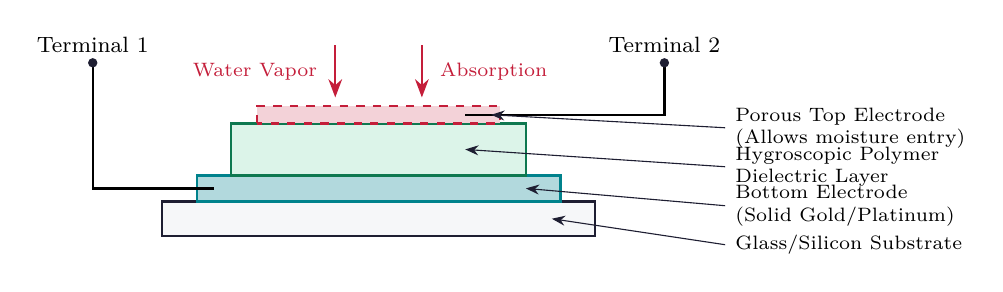
\begin{tikzpicture}[scale=1.1, thick, font=\small, >=Stealth]
  % Draw layers
  % Substrate (Glass/Silicon)
  \draw[fill=mygray, draw=mydark] (0, 0) rectangle (5, 0.4) coordinate (sub_mid);
  
  % Bottom Electrode (Solid Gold/Platinum)
  \draw[fill=myteal!30, draw=myteal] (0.4, 0.4) rectangle (4.6, 0.7) coordinate (bot_mid);
  
  % Dielectric Polymer Layer
  \draw[fill=hdrgreen, draw=mygreen] (0.8, 0.7) rectangle (4.2, 1.3) coordinate (poly_mid);
  
  % Top Electrode (Porous)
  \draw[fill=myred!20, draw=myred, dashed] (1.1, 1.3) rectangle (3.9, 1.5) coordinate (top_mid);

  % Terminals and contacts
  % Terminal 1 (Left - connected to Bottom Electrode)
  \draw (0.6, 0.55) -- (-0.8, 0.55) -- (-0.8, 2.0) node[circle, fill=mydark, inner sep=1.2pt] {} node[above] {\footnotesize Terminal 1};
  
  % Terminal 2 (Right - connected to Top Electrode)
  \draw (3.5, 1.4) -- (5.8, 1.4) -- (5.8, 2.0) node[circle, fill=mydark, inner sep=1.2pt] {} node[above] {\footnotesize Terminal 2};

  % Water Vapor / Absorption arrows
  \draw[redarrow] (2.0, 2.2) -- (2.0, 1.6) node[midway, left=0.1cm, font=\scriptsize\color{myred}] {Water Vapor};
  \draw[redarrow] (3.0, 2.2) -- (3.0, 1.6) node[midway, right=0.1cm, font=\scriptsize\color{myred}] {Absorption};

  % Callout Labels with leader lines (on the right/left)
  % We can place callouts on the right with a line pointing to each layer
  \node[anchor=west, align=left, font=\scriptsize] (lbl_top) at (6.5, 1.25) {Porous Top Electrode\\(Allows moisture entry)};
  \draw[->, thin, color=mydark] (lbl_top.west) -- (3.8, 1.4);

  \node[anchor=west, align=left, font=\scriptsize] (lbl_poly) at (6.5, 0.8) {Hygroscopic Polymer\\Dielectric Layer};
  \draw[->, thin, color=mydark] (lbl_poly.west) -- (3.5, 1.0);

  \node[anchor=west, align=left, font=\scriptsize] (lbl_bot) at (6.5, 0.35) {Bottom Electrode\\(Solid Gold/Platinum)};
  \draw[->, thin, color=mydark] (lbl_bot.west) -- (4.2, 0.55);

  \node[anchor=west, align=left, font=\scriptsize] (lbl_sub) at (6.5, -0.1) {Glass/Silicon Substrate};
  \draw[->, thin, color=mydark] (lbl_sub.west) -- (4.5, 0.2);
\end{tikzpicture}
\end{tcolorbox}

\subsubsection{Moisture Sensors}
Moisture measurement in materials (such as soil, paper, wood, or grain) is critical for industrial quality control and agriculture.
\begin{itemize}[leftmargin=*, itemsep=3.5pt]
  \item \textbf{Electrical Conductivity (Resistive) Method:}
    \begin{itemize}[leftmargin=*, itemsep=2.5pt, topsep=0pt]
      \item Operates by measuring electrical resistance between two metallic probes inserted into the material.
      \item Water is much more conductive than dry soil or organic fibers. Higher moisture content decreases resistance ($R \propto 1/\text{Moisture}$).
    \end{itemize}
  \item \textbf{Microwave Attenuation Method:}
    \begin{itemize}[leftmargin=*, itemsep=2.5pt, topsep=0pt]
      \item A microwave beam is transmitted through the material.
      \item Because water molecules have strong electric dipoles, they rotate rapidly in the microwave field, absorbing microwave energy.
      \item The attenuation (signal loss) and phase shift of the received signal are directly proportional to the total moisture content.
      \item This provides a non-contact, non-destructive, and continuous bulk measurement.
    \end{itemize}
\end{itemize}

\newpage
% ===============================================================================
\section{Data Acquisition Systems (DAS)}
% ===============================================================================

Data Acquisition Systems interface physical sensors with computers to measure and process parameters automatically.

\subsection{Analog and Digital DAS}
\begin{itemize}[leftmargin=*, itemsep=3.5pt]
  \item \textbf{Analog DAS:} Collects and displays data in continuous analog form (e.g., strip chart recorders, oscilloscope traces).
  \item \textbf{Digital DAS:} Converts analog signals into digital values for computer storage, display, and processing.
\end{itemize}

\begin{tcolorbox}[tikzbox, title={Digital Data Acquisition System Block Diagram}]
\centering

\begin{tikzpicture}[node distance=0.5cm and 0.8cm, thick, font=\scriptsize]
  \tikzset{
    sblock/.style={rectangle, draw=myteal, fill=hdrteal, text width=1.6cm, align=center, minimum height=0.8cm, rounded corners=2pt}
  }
  \node[sblock, fill=hdrred, draw=myred] (sensor) {Sensors\\(Transducers)};
  \node[sblock, right=0.7cm of sensor] (cond) {Signal\\Conditioners};
  \node[sblock, right=0.7cm of cond] (mux) {Analog\\Multiplexer};
  \node[sblock, right=0.7cm of mux] (sh) {Sample \&\\Hold (S/H)};
  \node[sblock, right=0.7cm of sh] (adc) {ADC};
  \node[sblock, right=0.7cm of adc, fill=hdrgreen, draw=mygreen] (pc) {Digital\\Computer};

  % Paths
  \draw[arrow] (sensor) -- (cond);
  \draw[arrow] (cond) -- (mux);
  \draw[arrow] (mux) -- (sh);
  \draw[arrow] (sh) -- (adc);
  \draw[arrow] (adc) -- (pc);
  
  % Input indicator
  \draw[arrow] ($(sensor.west) - (0.8, 0)$) -- node[above, font=\tiny] {Physical Input} (sensor.west);
\end{tikzpicture}
\end{tcolorbox}

\subsection{Roles of Key Digital DAS Components}
\begin{itemize}[leftmargin=*, itemsep=4pt]
  \item \textbf{Analog Multiplexer (MUX):} Sequences through multiple sensor channels, connecting one signal at a time to the common measurement chain. This avoids replicating expensive S/H and ADC components for every channel.
  \item \textbf{Sample and Hold (S/H) Circuit:} Captures the rapidly changing analog voltage at a specific instant and holds it constant at its output. This prevents errors during the time the ADC takes to perform a conversion.
  \item \textbf{ADC (Analog-to-Digital Converter):} Converts the held analog voltage into a proportional binary number (digital word) for the computer.
\end{itemize}

\newpage
% ===============================================================================
% MANDATORY QUICK REVISION PAGE
% ===============================================================================
\begin{center}
  {\large\bfseries\color{myred} Quick Revision --- Module 5}\\[3pt]
  {\small\color{mydark} Bridges, Parameter Measurement \& DAS $|$ OE-EC604A}
\end{center}
\noindent{\color{myred}\rule{\linewidth}{1.2pt}}
\vspace{4pt}

\begin{tcolorbox}[formulabox, title={\textbf{Key Module 5 Formulas}}]
\begin{align*}
  \text{Wheatstone Bridge:} \quad & R_x = \frac{Q}{P} R \qquad \text{Kelvin Double Bridge:} \quad R = \frac{P}{Q} S \ \left(\text{when} \ \frac{P}{Q} = \frac{p}{q}\right) \\
  \text{Maxwell } L_x: \quad & L_x = R_2 R_3 C_4 \qquad \text{Maxwell } R_x: \quad R_x = \frac{R_2 R_3}{R_4} \\
  \text{EM Flow EMF:} \quad & E = B \cdot D \cdot v \qquad \text{McLeod Vacuum:} \quad P \approx \frac{a \cdot h^2}{V} \\
  \text{Capacitive Humidity:} \quad & C \approx C_0 (1 + \alpha \cdot \text{RH}) \qquad \text{Relative Humidity:} \quad \text{RH} = \frac{p_v}{p_s} \times 100\%
\end{align*}
\end{tcolorbox}

\begin{tcolorbox}[defbox, title={\textbf{One-Line Definitions}}]
\begin{itemize}[leftmargin=*, itemsep=2.5pt, topsep=0pt]
  \item \textbf{Kelvin Double Bridge:} A bridge with double ratio arms to eliminate contact and lead resistance errors.
  \item \textbf{Maxwell Bridge:} An AC bridge used to measure medium-Q coil inductance using standard capacitance.
  \item \textbf{Electromagnetic Flow Meter:} An inductive flow meter measuring conductive fluid speed via Faraday's Law.
  \item \textbf{Pirani Gauge:} A thermal conductivity vacuum gauge measuring pressure via filament heat loss.
  \item \textbf{McLeod Gauge:} A mercury-filled vacuum gauge that compresses low-pressure gas to measure it hydrostatically.
  \item \textbf{Relative Humidity (RH):} Percent ratio of actual water vapor pressure to saturation vapor pressure.
  \item \textbf{Sling Psychrometer:} Instrument measuring humidity via dry-bulb and wet-bulb thermometers.
  \item \textbf{Hygrometer:} Electronic sensor designed to measure humidity in the atmosphere.
  \item \textbf{Multiplexer (MUX):} A switch routing multiple analog input channels sequentially to a single output line.
  \item \textbf{Sample and Hold (S/H):} A circuit holding analog voltage constant during the ADC conversion interval.
\end{itemize}
\end{tcolorbox}

\begin{tcolorbox}[exambox, title={\textbf{Frequently Asked / Viva Questions}}]
\begin{enumerate}[topsep=0pt, label=\textbf{Q\arabic*.}, itemsep=5pt]
  \item \Q{Why does a standard Wheatstone bridge fail to measure low resistances accurately?}
    At low resistances ($< 1\,\Omega$), the resistance of the connecting leads and contact terminals is significant relative to the test resistance. These lead resistances add directly to the measured resistance in a Wheatstone bridge, introducing massive measurement errors.
  \item \Q{Show how the lead resistance is eliminated in a Kelvin double bridge.}
    By incorporating inner ratio arms $p$ and $q$, the balance condition becomes $R = \frac{P}{Q} S + \frac{q r}{p + q + r}(\frac{P}{Q} - \frac{p}{q})$. Setting the outer ratios equal to the inner ratios ($\frac{P}{Q} = \frac{p}{q}$) cancels the second term, eliminating the lead link resistance $r$.
  \item \Q{Derive the balance equations for a Maxwell inductance-capacitance bridge.}
    Setting the opposite arm impedances equal, we get $Z_1 = Z_2 Z_3 Y_4$. Expanding: $R_x + j\omega L_x = R_2 R_3 (\frac{1}{R_4} + j\omega C_4)$. Separating real and imaginary parts yields $R_x = \frac{R_2 R_3}{R_4}$ and $L_x = R_2 R_3 C_4$.
  \item \Q{What are the limitations of a Maxwell bridge?}
    It is restricted to medium-Q coils ($1 < Q < 10$). For high-Q coils, $R_4$ must be extremely large, which is physically impractical. For low-Q coils ($Q < 1$), the balance converges very slowly due to sliding balance issues.
  \item \Q{An AC Maxwell bridge has $R_2 = 1\,\text{k}\Omega$, $R_3 = 2\,\text{k}\Omega$, $C_4 = 0.1\,\mu\text{F}$, and $R_4 = 100\,\text{k}\Omega$. Find the unknown $R_x$ and $L_x$.}\\
    Given: $R_x = \frac{R_2 R_3}{R_4} = \frac{10^3 \times (2 \times 10^3)}{100 \times 10^3} = 20\,\Omega$.\\
    $L_x = R_2 R_3 C_4 = 10^3 \times (2 \times 10^3) \times (0.1 \times 10^{-6}) = 0.2\,\text{H}$.
  \item \Q{Explain the working of an electromagnetic flow meter.}
    It operates on Faraday's Law ($E = B D v$). A magnetic field is applied across a pipe. The flowing conductive liquid acts as a conductor, generating an EMF across flush electrodes that is directly proportional to the average flow velocity.
  \item \Q{What is the principle of a Pirani vacuum gauge?}
    It works on the principle that the thermal conductivity of a gas is proportional to its pressure at low pressure. As chamber vacuum increases, less heat is conducted away from the filament, raising its temperature and resistance.
  \item \Q{Derive the pressure formula for a McLeod gauge.}
    Initial volume $V$ at pressure $P$ is compressed to volume $V_2 = a \cdot h$. The final pressure is $P + h$. By Boyle's Law: $P V = (P + h) a h = P a h + a h^2$. Since $P \ll h$, $P V \approx a h^2 \implies P \approx a h^2 / V$.
  \item \Q{Explain the dry-bulb and wet-bulb temperature principle of a Sling Psychrometer.}
    The dry bulb measures ambient temperature, while the wet bulb (covered in a wet wick) undergoes cooling due to water evaporation during slinging. The evaporation rate, and thus the wet-bulb temperature drop, is inversely proportional to relative humidity. In dry air, the drop is large; at 100\% humidity, the dry and wet bulb temperatures are equal ($T_d = T_w$).
  \item \Q{How does a capacitive humidity sensor detect relative humidity?}
    It uses a porous top electrode and a hygroscopic polymer dielectric. Water vapor penetrates the polymer. Since water has a high dielectric constant ($\epsilon_r \approx 80$) compared to the dry polymer ($\epsilon_r \approx 3$), the sensor capacitance increases proportionally to relative humidity.
  \item \Q{What is the principle of the microwave attenuation method for moisture measurement?}
    Water molecules have strong electrical dipoles that absorb microwave energy. When microwaves pass through a material, the signal attenuation and phase shift are directly proportional to the moisture content, providing a non-destructive bulk measurement.
  \item \Q{Why is a Sample and Hold circuit necessary before the ADC in digital DAS?}
    An ADC requires a finite time to convert an analog voltage into a digital word. If the analog input changes during this conversion period, the ADC output will suffer from aperture error. The S/H holds the input constant during conversion.
  \item \Q{Compare McLeod Gauge and Pirani Gauge.}
    McLeod gauge is an absolute, mechanical gauge working by volume compression, providing manual/discrete readings independent of gas type. Pirani gauge is a relative, thermal gauge providing continuous electrical output dependent on gas conductivity.
  \item \Q{What is the role of an analog multiplexer in a multi-channel DAS?}
    It acts as a rotary switch to connect multiple analog inputs sequentially to a single shared S/H and ADC. This reduces cost by eliminating the need for separate ADCs for each channel.
\end{enumerate}
\tcbset{colbacktitle=mypurple, coltitle=white}
\end{tcolorbox}

\begin{tcolorbox}[tikzbox, title={McLeod Gauge vs Pirani Gauge Comparison}]
\renewcommand{\arraystretch}{1.4}
\par\noindent
\begin{tabularx}{\linewidth}{|B{2.2cm}|Y|Y|}
\hline
\textbf{Feature} & \textbf{\color{myred}McLeod Gauge} & \textbf{\color{myteal}Pirani Gauge} \\
\hline
\textbf{Principle} & Gas volume compression (Boyle's Law). & Thermal conductivity variation. \\
\hline
\textbf{Reading Mode} & Discrete/Manual (batch process). & Continuous electrical reading. \\
\hline
\textbf{Gas Dependency} & Independent of gas composition. & Highly dependent on gas type. \\
\hline
\textbf{Output Signal} & Hydrostatic column level (height $h$). & Electrical resistance change. \\
\hline
\textbf{Calibration} & Absolute gauge (no calibration needed). & Relative gauge (needs calibration). \\
\hline
\textbf{Range} & $10^{-6}\,\text{torr}$ to $10^{-2}\,\text{torr}$ & $10^{-4}\,\text{torr}$ to $1\,\text{torr}$ \\
\hline
\end{tabularx}
\end{tcolorbox}

\end{document}
